\section{Grundlegende Architektur des Testmodells}
\label{sec:modelArchitecture}

Um Hadoop mit der Selfbalancing"=Komponente mit den in \cref{sec:requirements} beschriebenen Anforderungen prüfen zu können, wird mithilfe des \ac{ss}"=Frameworks ein vereinfachtes Modell der relevanten \ac{YARN}"=Komponenten entwickelt.
Dieses \ac{YARN}"=Modell wird mithilfe des Treibers mit dem realen Cluster verbunden, was durch hierfür entwickelte Scripte gesteuert wird.
Daraus resultiert folgende Drei"=Schichten"=Architektur für das gesamte Testmodell:

\begin{figure}[h]
    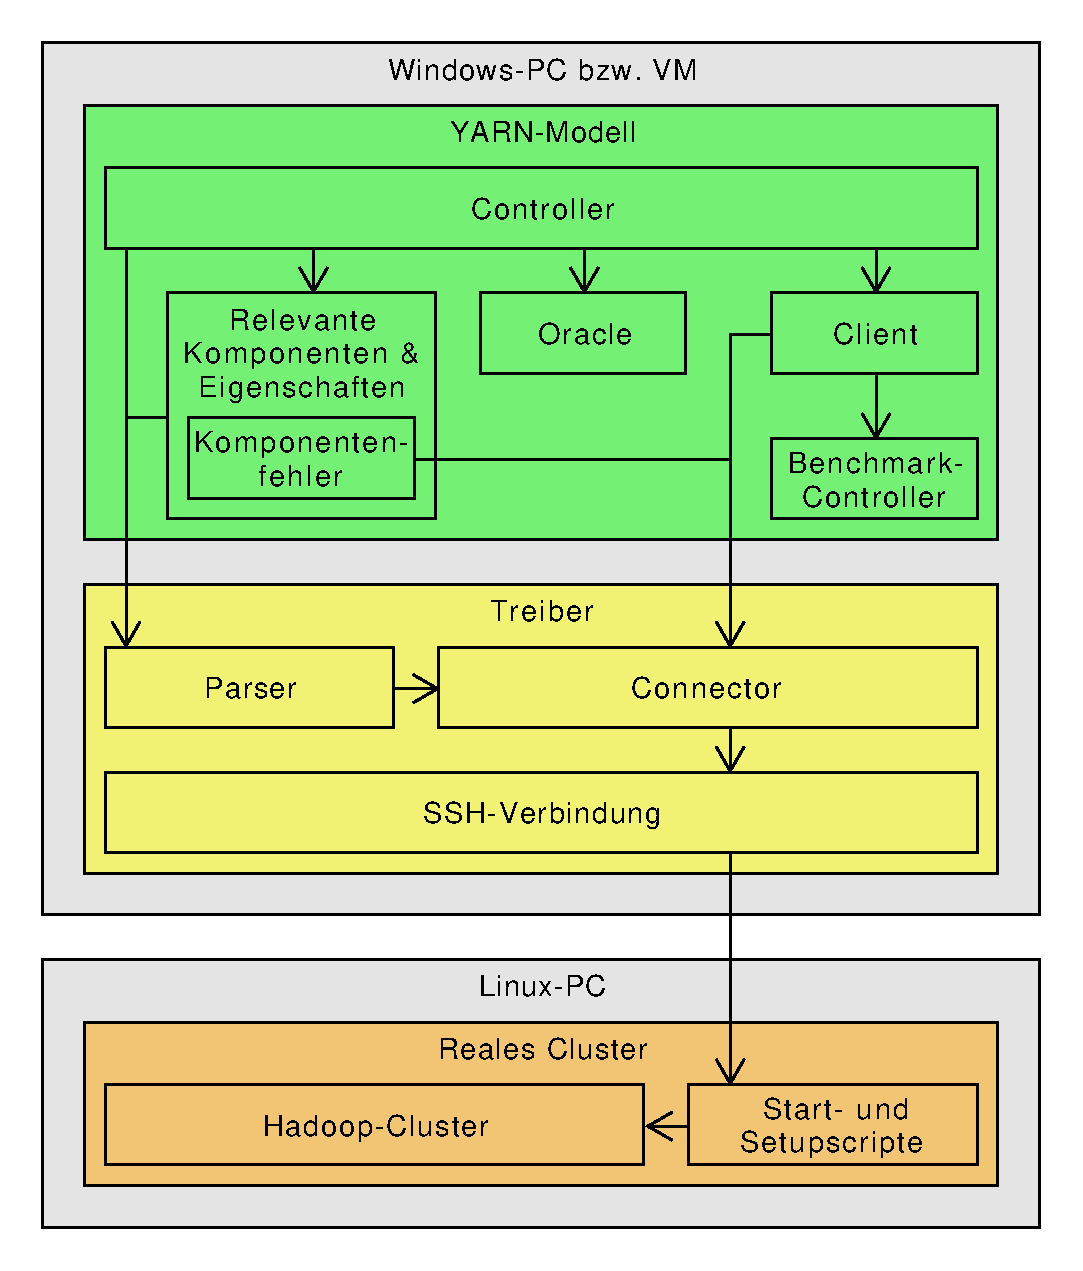
\includegraphics[width=0.6\columnwidth]{./resources/modelArchitecture.pdf}
    \caption{Grundlegende Architektur des Testsystems}
    \label{fig:modelArchitecture}
\end{figure}

Das \ac{YARN}"=Modell stellt die oberste Schicht des Testmodells dar.
Es bildet das Kernstück dieser Fallstudie, da dieses Modell mit den hierin abgebildeten, für diese Fallstudie relevanten \ac{YARN}"=Komponenten und implementierten Komponentenfehlern, dem Controller und dem Oracle direkt im Rahmen des modellbasierten Testens mit \ac{ss} interagiert.
Folgende Komponenten sind im \ac{YARN}"=Modell enthalten:

\begin{description}
    \item [Controller] \hfill \\
        Steuert den Ablauf einer Testausführung und das Zusammenspiel zwischen den Komponenten des \ac{YARN}"=Modells.
    \item [Relevante \ac{YARN}"=Komponenten und Eigenschaften] \hfill \\
        Bilden die grundlegende Architektur von Hadoop \ac{YARN} ab.
        Implementiert wurden in dieser Fallstudie die Nodes, Anwendungen, Attempts und Container mit den jeweils relevanten Eigenschaften zur Durchführung der Fallstudie.
    \item [Komponentenfehler der \ac{YARN}"=Komponenten] \hfill \\
        Bilden die bei den Tests zu injizierenden Komponentenfehler der jeweiligen \ac{YARN}"=Komponenten.
    \item [Oracle] \hfill \\
        Validiert die in Form von Constraints in den jeweiligen \ac{YARN}"=Komponenten implementierten Anforderungen.
    \item [Client] \hfill \\
        Dient zum starten und beenden von Benchmarks im Cluster.
    \item [Benchmark"=Controller] \hfill \\
        Enthält das Transitionssystem zur Auswahl der Benchmarks und steuert diese.
\end{description}

Die Verbindung zwischen dem \ac{YARN}"=Modell und dem realem Cluster bildet der Treiber.
Er besteht aus folgenden Komponenten:

\begin{description}
    \item [Parser] \hfill \\
        Verarbeitet die Monitoring"=Ausgaben vom realen Cluster und konvertiert diese für die Nutzung im \ac{YARN}"=Modell.
    \item [Connector] \hfill \\
        Abstrahiert die Verbindung zum realen Cluster und die dabei auszuführenden Befehle.
    \item [SSH"=Verbindung]  \hfill \\
        Stellt die Verbindung zum realen Cluster her.
\end{description}

Der Parser wird hierbei nur zur Durchführung des Monitoring benötigt und nutzt wiederum den Connector zum abrufen der Daten.
Andere Befehle und Zugriffe auf das reale Cluster, wie \zB das Injizieren von Komponentenfehlern, werden direkt mithilfe des Connectors durchgeführt.

Die Implementierung des \ac{YARN}"=Modells wird in \cref{sec:yarnModel} beschrieben, die Implementierung des Treibers in \cref{sec:sshDriver}.
Die Umsetzung des realen Clusters wird in \cref{sec:realCluster} beschrieben.

In allen Komponenten des Modells werden, sofern benötigt, mithilfe des Frameworks log4net\footnote{\url{https://logging.apache.org/log4net/}} (Version 2.0.8), Logausgaben getätigt.
Dies betrifft vor allem das Monitoring (vgl. \cref{subsubsec:yarnComponentInterface}), aber auch weitere Informationen wie zur Validierung der Constraints (vgl. \cref{subsec:oracleImpl}) oder reine Debug"=Informationen.
All diese Informationen werden im Programmlog zusammengefasst, welches auch zur Auswertung der ausgeführten Tests dient.
Zu Analysezwecken im Fehlerfall wird zudem jede Kommunikation der SSH"=Verbindung in einem eigenen Log, dem SSH"=Log, abgespeichert (vgl. \cref{subsec:sshConnection}).
